\textbf{Motivation}. 
In the 1940s, whooping cranes were almost completely extinct in the U.S., with only 20 existing in the wild~\citep{cannon1996whooping}. Thanks to efforts over the years to preserve their population, there are roughly 650 wild cranes today. This key species is still listed as endangered in 2025. %due to several threats.

%For example, Aerial Surveys were conducted from 1950-2011 to monitor the cranes’ ecological habits. \citep{asurv}
% and from 2009-2018, the United States Geological Survey group (USGS) tagged Whooping Cranes with GPS trackers to monitor the species’ wintering and breeding. 
%These ecological efforts to maintain the population have succeeded, with 650 cranes in the wild today. 

A major flock of cranes, known as the Aransas-Wood population, winters at the Aransas National Wildlife Refuge (ANWR) along the Gulf Coast of Texas~\citep{aransas_wood}, while spending summers north in Canada. 
Ecologists wish to actively monitor this population.
Regular aerial surveys of the Texas wintering region have been conducted for decades~\citep{asurv}.
Using binned spatiotemporal data of sighting counts over time from these surveys, we wish to offer data-driven forecasts of where cranes may be found. 
This could help conservationists decide where to send future human monitors or where to place $K$ fixed-location cameras to efficiently track population health.

% Manually monitoring the entirety of the Aransas-Wood population is infeasible. In a reality where ecologists aim to maximize the amount of cranes they can monitor on a limited budget, perhaps via fixed-location cameras or human observation, our top-K solution is well suited for this decision-making task.

\textbf{Data}. 
We use raw data from \citet{asurv}, which digitized decades of aerial surveys of ANWR that marked individual crane sightings on paper maps. % into a cohesive dataset.
We processed this \emph{ANWR TX Cranes} data into a common format of sighting counts over time and space, selecting bin sizes to support our goal of using the top-$K$ sites to improve monitoring.
Quality cameras or binoculars that could be used to track cranes can reasonably capture a 1.5 meter tall whooping crane in a 250-meter radius. Therefore, for spatial units, we divided the ANWR into 1338 boxes, each 500 meters per side. 
For temporal binning, we use 2 month periods.
This choice catches seasonal variation, but avoids how finer scales might burden staff to move cameras too often.

% we units. We believe this captures a scale short enough that the predictive task would be useful but long enough for researchers to comfortably monitor a different top-K sites every period, perhaps by moving cameras every two months. 


%We study the capabilities of the top-K ranking and training methods on two datasets: Aerial Surveys and GPS tracking. Starting in 1950 until 2011, aerial surveys of the Aransas National Wildlife Refuge (NWR) were conducted to keep track of Whooping Crane abundance. In February 2015, Taylor et. al. \citep{asurv} digitized these aerial surveys into a cohesive dataset; previously, the survey information was only contained by paper maps. From the digitization, the researchers were able to create a dataset with each row corresponding to a location-timestamp observation of one or more Whooping Cranes. 


%For each dataset, we calculated the observed number of Whooping Cranes at timestep t in location s. Each dataset included a consistent set of covariates for predictive modeling. At each bimonth ttt and spatial division sss, the following were provided: historical bird counts, the latitude and longitude of the box’s centroid, and the timestamp (the number of “bimonths” since the first year). 


% MCH: commented out GPS data, not gonna use for now
%From 2009-2014, Pearse et. al. marked 68 Whooping Cranes from the Aransas population (about 12\% of the total Aransas population) with a GPS tracker. From 2009 until 2018, their team tracked the locations of these Cranes every six hours, compiling the results into a dataset with a similar location-timestamp indexing as the Aerial Surveys. Although 68 birds is a seemingly low quantity, in 2023 there existed only 536 Cranes in the Aransas-Wood population, so the 68 marked Cranes comprise a substantial percentage of the full population. \cite{2223update}\cite{fws}For this dataset and Aerial Surveys, we choose K=75 sites out of 2,156 total sites.

\textbf{Task}. The experiment on these data was trained on years 2002-2006, validated on 2007-2008, and tested on 2009-2010. In this context, a "year" represents one wintering season; winter 2010 means the winter that began in October 2010 and ended in April 2011.
We choose $K=50$ for this task. This is an estimate of how many sites scientists might reasonably monitor every two months on a limited budget.

%We believe that 50 sites is an adequate amount for scientists interested in studying Whooping Crane's ecological habits.

%Below, we present two datasets suitable for a top-K machine learning problem: Aerial Survey data and GPS tracking data of Whooping Cranes. \cite{source1} \cite{source2} The Aerial Survey data lasts far longer than the GPS tracking data–50 years in contrast to 9 years–but the GPS tracking data is far more precise and less sparse than the Aerial Survey data. As such, both datasets have unique strengths and are suitable for a top-K machine learning task.

\textbf{Models}. The same negative binomial mixed-effect model was used as in Sec.~\ref{sec:results_opioid}. Features $\bm{x}_{st}$ for site $s$ at time $t$ include historical bird counts at $s$, the latitude and longitude of the site's centroid, time of year, and the overall time.

\textbf{Setup}. We followed the common setup described above.
See reproducible details in App.~\ref{supp:results_birds}.

%The same training objectives and hyperparameter search efforts were used as in Sec.~\ref{sec:results_opioid}.

\textbf{Results.} From results in Fig.~\ref{fig:Frontier} (right panel), we find that optimizing NLL or BPR \emph{alone} will yield poor results in the other metric. In this case, direct optimization of BPR results in the best top-K decisions, but dramatically worse likelihood. Our DAML models improve BPR by up to 0.05 over conventional ML training with only modest decay in likelihood. 
Our DAML and direct BPR objectives also deliver better BPR than previous decision-aware methods (PG, SPO+). 
This is even after providing smarter initializations to these methods, as we found their training had trouble improving on our common random initialization of $\phi$, perhaps due to this task's much sparser $\bm{y}$ values.

%Due to the task's sparsity, we found the surrogate losses to require a careful initialization in order to learn. 
%Given that BPR is the most relevant performance metric for this real-world task, our findings support the DAML objective as the best model for real-world impact without losing considerable log likelihood.



% MCH: this was subsumed by the new Fig 4 that combines all real results
% \begin{figure}
% \begin{tabular}{c}
% 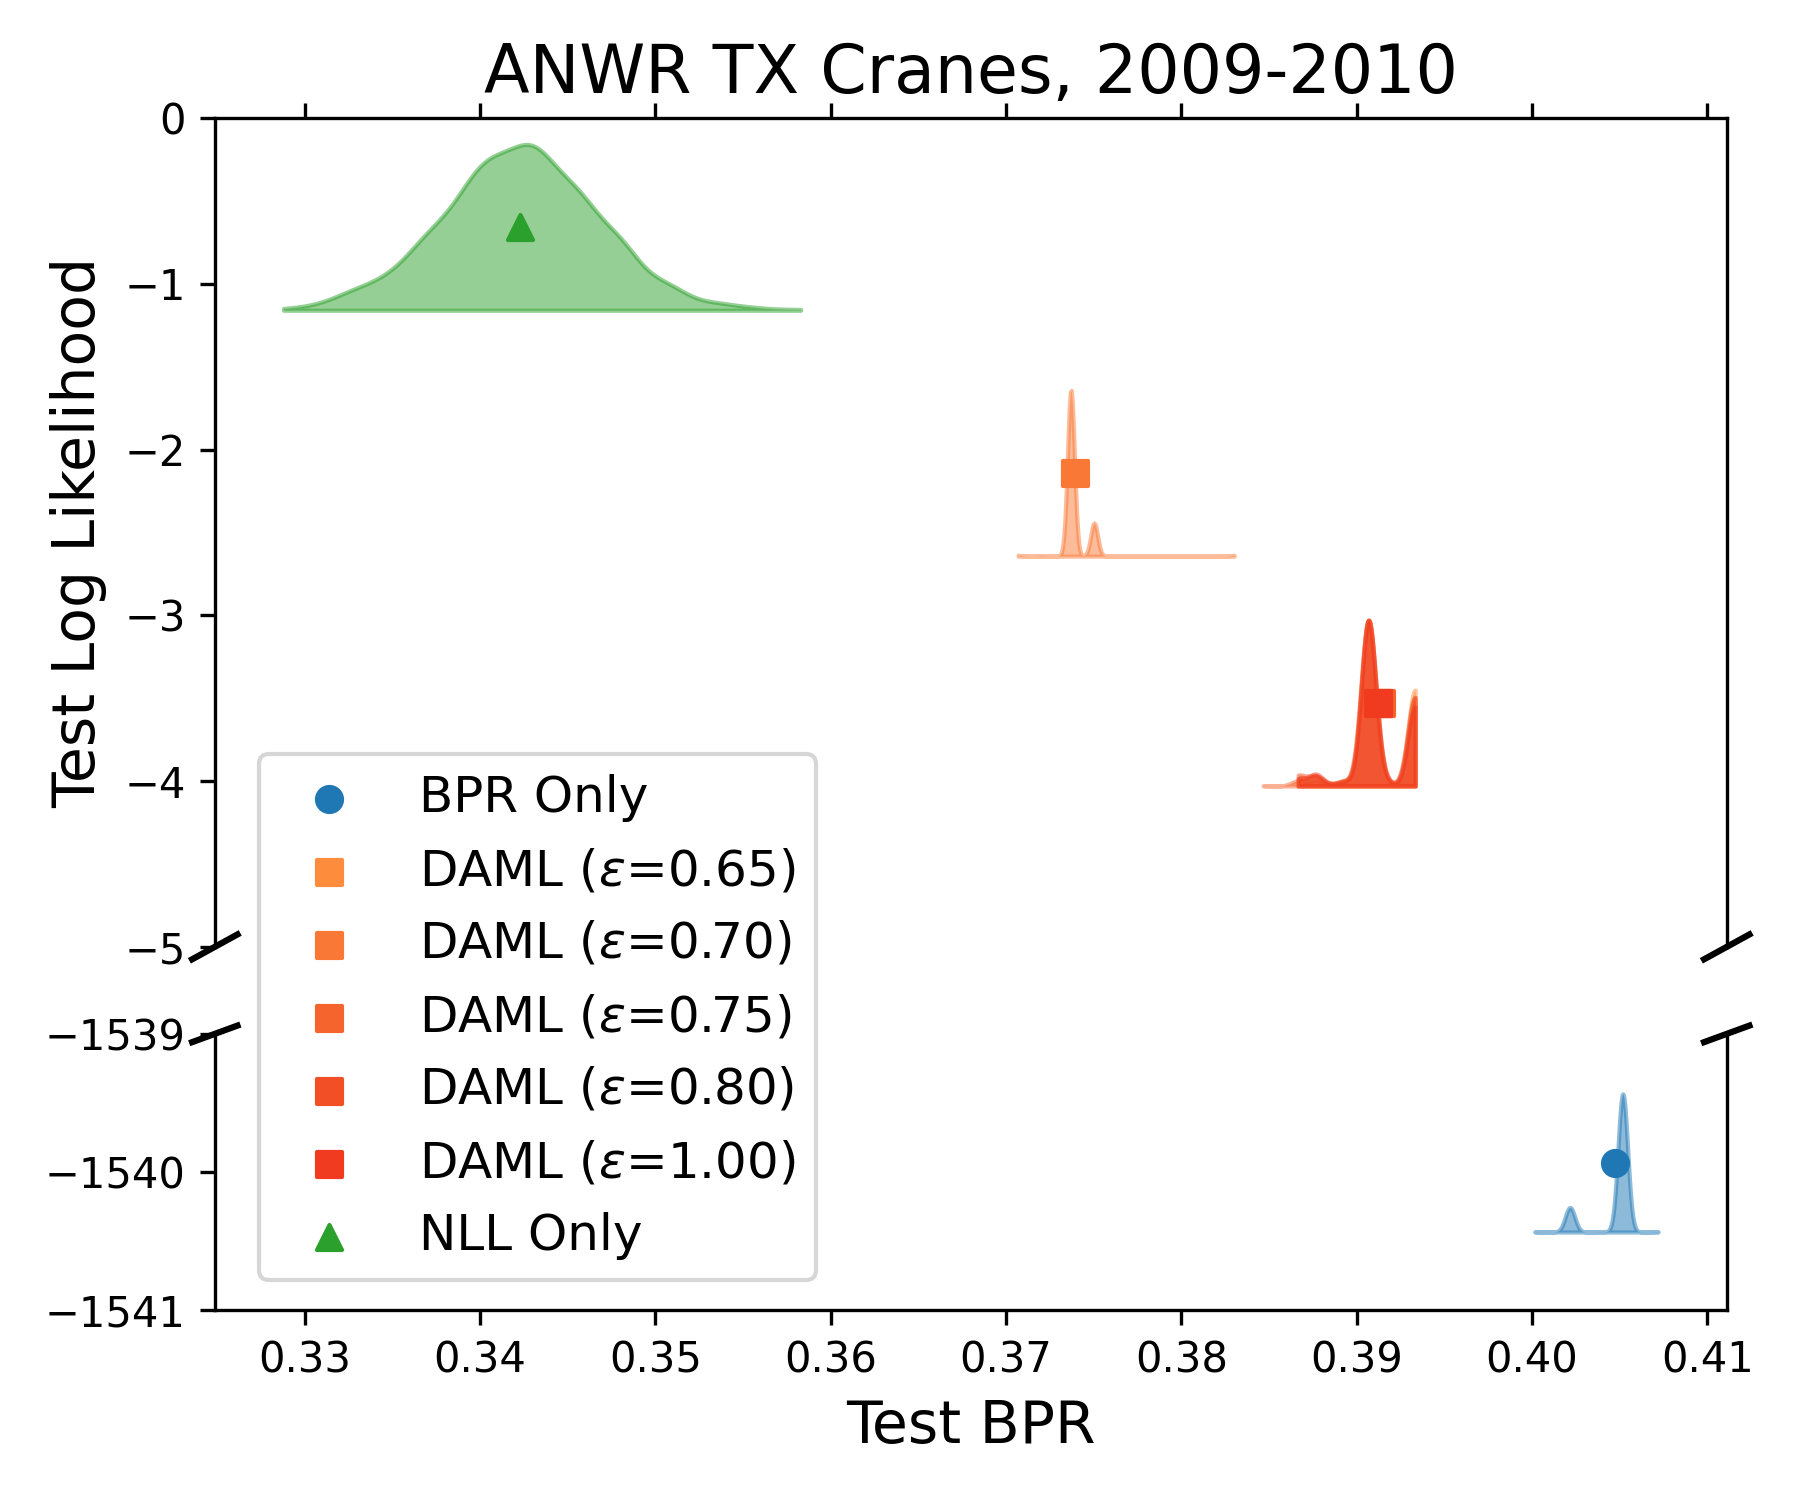
\includegraphics[width=.5\textwidth]{figures/AsurvTest.png}
% \end{tabular}
% \captionof{figure}{
% \textbf{Results on heldout aerial survey data}.
% }%end caption
% \label{fig:bird_results}
% \end{figure}
